\documentclass[10pt,red]{beamer} 
% change the alerted colour to blue
\setbeamercolor{alerted text}{fg=blue}

\usetheme{berlin}
% theme split
\usepackage{beamerthemesplit}

\usepackage{booktabs,array,}
\usepackage{listings}
\usepackage{hyperref}
\usepackage{verbatim,moreverb}
\usepackage{tikz}

\usepackage{color}

\definecolor{dkgreen}{rgb}{0,0.6,0}
\definecolor{gray}{rgb}{0.5,0.5,0.5}
\definecolor{mauve}{rgb}{0.58,0,0.82}

\lstset{frame=tb,
  language = Java,
  aboveskip=3mm,
  belowskip=3mm,
  showstringspaces=true,
  columns=flexible,
  basicstyle={\small\ttfamily},
  numbers=none,
  numberstyle=\tiny\color{gray},
  keywordstyle=\color{blue},
  commentstyle=\color{dkgreen},
  stringstyle=\color{mauve},
  breaklines=true,
  breakatwhitespace=true
  tabsize=4
}
% theme shadow
\usepackage{beamerthemeshadow}

% For including figures
\usepackage{graphicx}

% logo
\logo{
\includegraphics[height=1cm]{iitblogo.pdf}}


% sf family, bold font
\sffamily \bfseries
% Beginning of title page
\title
% content inside [] appears at bottom of all page. content inside {} appears on first page as title. double backslash means line change 
[
	Raspberry Pi Hardware Development	% bottom
	\hspace{0.5cm}
	\insertframenumber/\inserttotalframenumber
]
{
	Interfacing Port Expander MCP23017 IC
}

\author
[
	www.e-yantra.org
]
{
	e-Yantra Team \\
  Embedded Real-Time Systems Lab\\
  Indian Institute of Technology-Bombay \\
}
\date
{
IIT Bombay \\ {\today}
}
 
 
\begin{document} 

% Slide-1: Title Page
\begin{frame}
	\titlepage
\end{frame}
\section{Port expander}
\begin{frame}
	\frametitle{Port Expander} \pause
	\textcolor{blue}{Function:} \pause
	\text{It is used to increase IO pins of microcomputer.} \pause
	\begin{itemize}
		\item<+-|alert@+> Since there are only 26 GPIO pins available on Raspberry Pi.
		\item<+-|alert@+> Port expander is used to increase GPIO pins of Raspberry Pi.
	\end{itemize}
\end{frame}
\begin{frame}
	\frametitle{About MCP23017 IC} \pause
	\begin{enumerate}
		\item<+-|alert@+> It is a 28 pin IC.
		\item<+-|alert@+> It consists of two ports having 8 pins each available for GPIO.
		\item<+-|alert@+> It uses I2C protocol to communicate with Raspberry Pi.
		
	\end{enumerate}
	
\end{frame}
\begin{frame}
	\frametitle{Pins of MCP23017} \pause
	\centering
	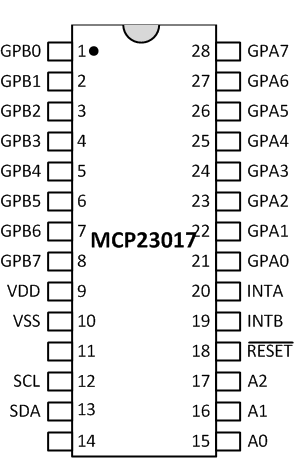
\includegraphics[scale = 0.6]{mcp23017}
\end{frame}
\section{Experiment}
\begin{frame}
	\frametitle{Experiment} \pause
	\textbf{Interfacing an LED and switch to Raspberry Pi using MCP23017 IC}
\end{frame}
\begin{frame}
	\frametitle{Hardware required for the experiment:} \pause
		\begin{tabular}{c c c c }
			 1.  & Breadboard & & 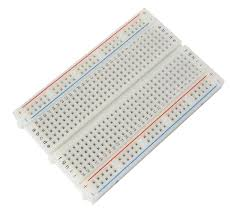
\includegraphics[scale = 0.2]{breadboard} \\ \pause
			 2.  & MCP23017 IC & & 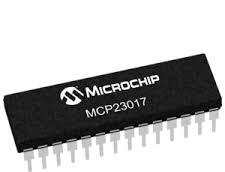
\includegraphics[scale = 0.2]{mcp23017_ic} \\ \pause
			 3.  & Switch	& &	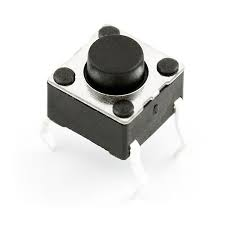
\includegraphics[scale = 0.1]{push_button} \\ \pause
			 4.  & LED 		&  &	
\includegraphics[scale = 0.2]{led} \\  \pause
			 5.  & 330 ohm resistor & &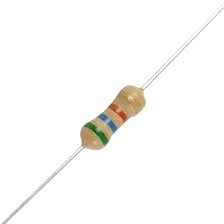
\includegraphics[scale = 0.1]{resistor}  \\
		\end{tabular}
\end{frame}
	\begin{frame}
		\frametitle{Connections:} \pause
		\centering
		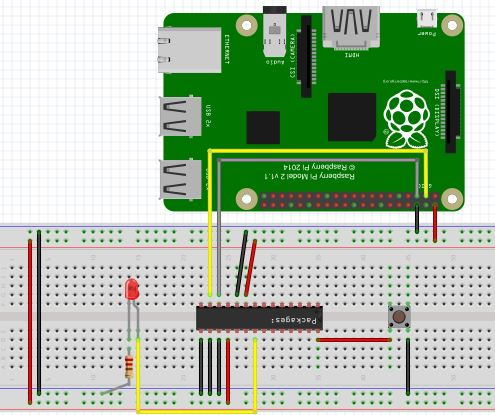
\includegraphics[scale=0.6]{mcp23017_connection}
	\end{frame}
	
\subsection{Problem Statement}
\begin{frame}
	\frametitle{Problem Statement} \pause
	\textbf{Turn on the LED for 1 second when button is pressed.}
\end{frame}
\begin{frame}
	\hskip4cm
	\textbf{\LARGE Thank You!} \\[20pt]
	\hskip3cm
	\scriptsize Post your queries on: 
	\hyperref[www.e-yantra.org]{\color{blue} http://qa.e-yantra.org/ \color{black}} 
\end{frame}
\end{document}